% define document type (i.e., template. Here: A4 APA manuscript with 12pt font)
\documentclass[man, 12pt, a4paper]{apa7}

% add packages
\usepackage[american]{babel}
\usepackage[utf8]{inputenc}
\usepackage{csquotes}
\usepackage{hyperref}
\usepackage[style=apa, sortcites=true, sorting=nyt, backend=biber, natbib=true, uniquename=false, uniquelist=false, useprefix=true]{biblatex}
\usepackage{authblk}
\usepackage{graphicx}
\usepackage{setspace,caption}
\usepackage{subcaption}
\usepackage{enumitem}
\usepackage{lipsum}
\usepackage{soul}
\usepackage{xcolor}
\usepackage{fourier}
\usepackage{stackengine}
\usepackage{scalerel}
\usepackage{fontawesome}
\usepackage[normalem]{ulem}
\usepackage{longtable}
\usepackage{amsmath}
\usepackage{afterpage}
\usepackage{float}
\usepackage{titling}
\usepackage{censor}

% formatting links in the PDF file
\hypersetup{
pdfpagemode={UseOutlines},
bookmarksopen=true,
bookmarksopenlevel=0,
hypertexnames=false,
colorlinks   = true, %Colours links instead of ugly boxes
urlcolor     = blue, %Colour for external hyperlinks
linkcolor    = blue, %Colour of internal links
citecolor   = cyan, %Colour of citations
pdfstartview={FitV},
unicode,
breaklinks=true,
}

% language settings
\DeclareLanguageMapping{american}{american-apa}

% add reference library file
\addbibresource{references.bib}

% Title and header
\title{Supplemental Information A: Context of the Migration Experience Framework}
\shorttitle{SI A: Acculturation Context}
\author{Jannis Kreienkamp, Laura F. Bringmann, Raili F. Engler, Peter de Jonge, Kai Epstude}

% set indentation size
\setlength\parindent{1.27cm}

% adapt table and figure labels
\setcounter{equation}{0}
\setcounter{figure}{0}
\setcounter{table}{0}
\setcounter{page}{1}
\makeatletter
\renewcommand{\theequation}{S\arabic{equation}}
\renewcommand{\thefigure}{S\arabic{figure}}
\renewcommand{\thetable}{S\arabic{table}}

% Start of the main document:
\begin{document}

% add title information (incl. title page and abstract)
\begin{titlepage}
	{\noindent\Large Supplementary Information for \par}
	\vspace{0.5cm}
	{\noindent\Large The Migration Experience: A Conceptual Framework and Systematic Review of Psychological Acculturation\par}
	\vspace{1.5cm}
	{\noindent\LARGE\bfseries \thetitle \par}
	\vspace{2cm}
	{\noindent\Large\itshape \theauthor \par}
	\vfill
	\noindent Corresponding Author Jannis Kreienkamp\par
	\noindent E-mail: j.kreienkamp@rug.nl\par
	\vfill

    % Bottom of the page
	{\noindent Last updated: \today\par}
\end{titlepage}

% add title again on page 1 (after title page)
\begin{center}
   \textbf{\thetitle} 
\end{center}

This supplementary information elaborates on the background literature of the contextual aspects of our conceptual framework presented in the main text. We would like to address each of the four contextual factors in more detail: (1) Cultures, (2) individuals, and (3) situations.

\begin{figure}[h]
\centering
\caption{Conceptual Model with Context.}
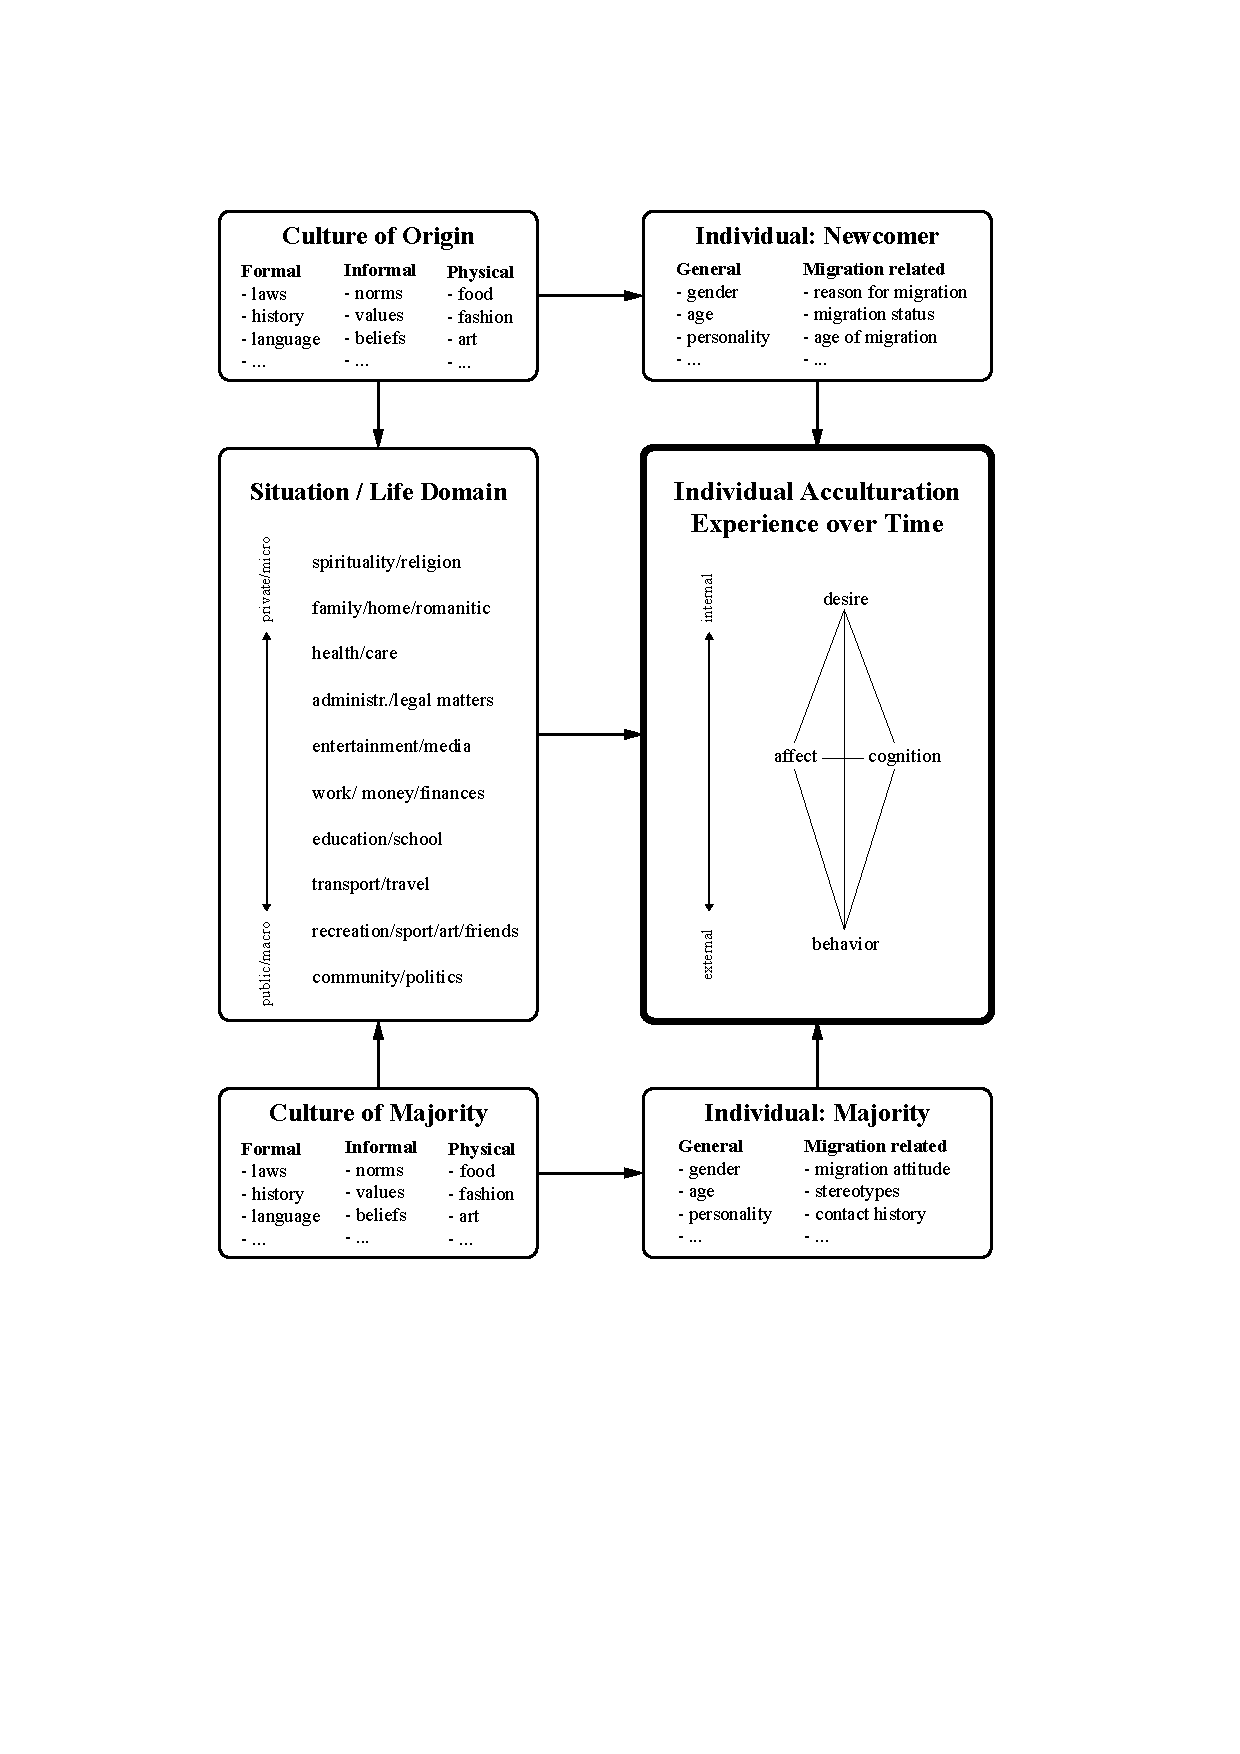
\includegraphics[width=\textwidth]{Figures/ConceptualFrameworkStatic.pdf}
\label{fig:SupModelContext}
\end{figure}

\section{Culture} 
% Culture as social facts and Cultural adaptation as tension between different social facts.
The most prominent contextual factor of psychological acculturation is probably the concept of culture. Functional structuralists, who tried to structure the concept of culture, have defined culture as external social expectations focused on our "manners of acting, thinking and feeling, which are invested with a coercive power by virtue of which they exercise control over him" \citep[][p. 52; on social facts]{Durkheim1982, Gilbert1989}. Within the sociological literature, these social influences can be divided into the formal social facts (e.g., laws, regulations, policies, history, language), informal social facts \citep[e.g., norms, values, beliefs, rituals, customs; also see][]{Herzog2018}, as well as more material cultural products or artifacts \citep[e.g., food, fashion, architecture, or arts, such as film, music, literature, and fine arts; e.g., see][]{Alexander2001}. The content of these external influences will likely be relevant in the expected patterns of behavior (e.g., dress or communication styles), cognition (e.g., sense of race-, class-, gender-, and sexual identities), emotions (e.g., expressions of emotions), and motivations (e.g., virtues and duties).

At the same time affect, behaviors, cognitions, and desires also drive what we consider `cultures' to be \citep[e.g.,][]{Varnum2017}. For example, cultural knowledge, values, identities, beliefs, and attitudes are likely the most widely discussed aspects of non-material culture \citep[e.g.,][]{DiMaggio1997}, some indigenous cultural practices are legally protected as manifestations of culture \citep[Art. 11]{UnitedNations2007}, shared emotions are an integral part of culture creation in narratives \citep[e.g.,][]{Ahmed2014, Kitayama1994, Smith2016c, Sundararajan2015}, and motivational ideals or oughts form the basis of many cultural discussions \citep[e.g., see][]{Markus1991}.

In the case of psychological acculturation, an individual needs to deal with (at least) two sets of cultural expectations --- their heritage culture and the culture of the new environment \citep[e.g., see models of][]{Berry1997b, Berry2006a}. The individual will thus have to negotiate their individual response to the cultural expectations by their heritage and host culture. Once we consider culture as external influences on emotions, behaviors, cognitions, and desires and psychological acculturation as the individual adjustments to the presence of multiple cultural influences, it becomes apparent that the experience framework may be ideally suited to discuss the concept of culture. The psychological acculturation experience (i.e., the individual experience of ABCD) allows one to capture the adjustment to tension as a result of differing external expectations of affect, behavior, cognition, and desire. Studying psychological acculturation in the experience framework then also allows us to reflect on which cultures' social expectations are considered in the conceptualization of acculturation \citep{Bhatia2001}. 

As part of the analyses presented in this paper, we will offer such a reflection by extracting the cultures for which acculturation measures were validated and investigated in empirical papers. This allows us to examine how much the external influences of culture on motives, emotions, thoughts, and behaviors are reflected within structural differences of measures and definitions (that is, if we can consolidate a meaningful number of studies per cultural context).

\section{Individual} 
%% Individual based on inter-group contact and Berry: 
% Individual differences in general (e.g., age, gender) but also migration related differences (e.g., reason for migration, language proficiency)
Another contextual factor to consider during the cultural adaptation process are the interacting individuals themselves. There has been a rising focus on the idea that acculturation centers around the daily interpersonal interactions a person has with people of the other group \citep{Maxwell2017, Sam2010}. And although it can, at times, be difficult to disentangle cultural from individual influences, there are a range of personal features that likely influence the cultural adaptation process. These personal differences might relate to relatively stable individual differences, such as gender or personality, but also migration related differences, such as the reason for migration (e.g., voluntary vs. forced migration), cultural distance, or migration status. Within the migration related factor we would also include aspects that might change over the course of the adaptation process but give migrants different starting positions, such as language skills and education level.
Similar to the influences of cultures, the individual differences of the interaction partners (if there are multiple people) will likely impact the cultural adaptation. And similar to culture, individual differences likely play a role for multiple aspects of the cultural adaptation process (also see Figure \ref{fig:SupModelContext}). As part of this study, we will mainly analyze the migration relevant differences. Considering individual differences on a larger, cross-study level we will mainly extract data on the type of samples collected within the validation and the empirical papers (e.g., forced vs. voluntary, youth, or clinical samples). If we find reasonable numbers of studies with specific types of samples, we will assess whether these individual differences are related to structural differences in measures or definitions used by the authors.

\section{Situation} 
%% Situations as domains of psycho-social functioning: 
% Many theories have come up with life domains that form different cultural interaction situations.
Beyond the cultural group and the individuals, the interactions of cultural adaptation are further dependent on the situational context. One way of structuring this situational context is what we will here refer to as the \textit{domains of psycho-social functioning} -- the idea that the social experience will take place within different domains in life. There are many social-scientific theories that have discussed these spheres of life. One famous example is Bronfenbrenner's Ecological systems theory \citep{Bronfenbrenner1992}, according to which humans get into contact with others, and society at large, through a number of environmental systems that range from the closest relations (e.g., family or colleagues) to the more remote relationships (e.g., mass media or societal services). A similar framework was suggested by prominent theorists of the (structural) functionalist traditions with the concept of social institutions \citep[e.g.,][]{Turner1997}. According to these sociological theorists, it is through societal institutions (commonly: family, government, economy, media, education, healthcare, and religion) that culture is transmitted and maintained \citep[e.g.,][]{Durkheim1982}. Similar ideas for domains of interaction with society and culture have also been proposed within the acculturation literature. \citet{Arends-Toth2006, Arends-Toth2007} have, for example, suggested 15 public and private life domains (e.g., education [public], child-rearing [private]) in which acculturation takes place. Empirical research in the individual acculturation field, have also provided evidence that acculturation processes can develop separately and differently within these situational domains \citep[e.g.,][]{Arends-Toth2003a}. 

%% Point of convergence: 
% We aggregate a list of micro to macro domains from past literature.
What structurally unites the conceptualizations of life domains is the dimension of closeness to the individual. That is, most areas of life found in the literature can be arranged from the most immediate (i.e., micro or private, such as family) to the broadest levels (i.e., macro or public, including government or media). So, based on sociological theories of social institutions \citep{Durkheim1982}, literature on life domains in acculturation \citep{Arends-Toth2006, Arends-Toth2007, Zane2004}, a categorization of psychological influences by the British Psychological Society \citep{Michie2005a}, and Bronfenbrenner's Ecological systems theory \citep{Bronfenbrenner1992}, we conceptualized a range of life domains relevant to the migration process (also see Figure \ref{fig:SupModelContext}). Interestingly, most methodological and empirical authors mention explicitly which domains of acculturation they measure or very clearly focus on a limited number of domains in their measurement or definition of acculturation. As part of this study we will, therefore, extract information on the domains mentioned and measured in the literature. We will then assess whether different foci on life domains also show differences in their understanding and measurement of the motivational, emotional, cognitive, and behavioral cultural adaptation.

\section{Measurement}
As part efforts to capture the migration context we were interested in cultural, individual, situational, as well as process related contexts. Assessing these contexts in a manner that is relevant across a wide range of studies is challenging and likely superficial at best. Context is arguably more relevant if one considers a single case, yet gaining a more general understanding of the contexts frequently considered in the literature could prove useful in evaluating and comparing conceptions of cultural adaptation. We, thus, extracted a range of general context variables from the empirical literature.

\subsection{Cultural Context}
To capture the cultural contexts researched, we coded both the heritage country of the migrants as well as the country of the receiving host society. Coding the two societal contexts allows us to extract information on the specificity of the studies (e.g., Mexican migrants in the United States, vs any migrant in Scandinavia). Migrant and host country coding could also reveal patterns of interest within the literature (e.g., common migrant groups, common host societies, or common combinations investigated). And finally, if common clusters emerge, we could compare the types of experience elements assessed within each cluster (e.g., focus on behavioral adaptation in one and cognitive focus in another cluster). 

\subsection{Sample}
To capture the individual background on a cross-paper level, we extract the types of samples recruited by the authors. Some studies might focus on young or elderly samples, men or women only, clinical samples, or authors might simply recruit any migrant from a certain country or region. Clusters and differences in the experience foci within these clusters might offer insights into the understanding of cultural adaptation for different individual contexts.

\subsection{Life Domains}
To capture the situational focus of the authors, we coded which life domains the scales referred to. There were a range of ways in which we could identify the domains the authors wished to cover. Often times authors will explicitly mention which life domains their measure aims to capture. Others will mention clear domain focus as part of sub-scale or factor labels. If there is no explicit mention by the authors, questions are likely worded to refer to a specific life domain (e.g., behaviors at school, or values in the family context). If there is no clear reference to a life domain or the questions are about life in general, we code this as meaningful information as well. We can then process the situational foci as a list of domains, which offers information on the diversity of domains (e.g., number, or similarity of domains) but also the focus in the literature in general (e.g., frequency of domain across all articles). If clusters of similar focus domains emerge, we could, additionally, assess differences in the assessment of cultural adaptation for these clusters.

\section{Results}
% import methods and results from R Markdown (in file: "ContextResults.tex")
\subsection{Methodological Literature}

To gain a general understanding of contextual factors within the
validated studies, we also assessed cross-study patterns of cultural,
individual, situational, and process-related focus points.

\paragraph{Country}

To assess the cultural contexts for which scales were validated, we
assessed the migrants' countries of settlement as well as the countries
of origin. We found that most scales investigated a single host country
(\textit{N} = 195) and most investigated one country of origin
(\textit{N} = 134). There were only 29 scales that were validated for
more than one receiving country. Looking at the country patterns, we
found that an overwhelming number of scales were validated within a U.S.
American settlement context (\textit{N} = 124). But also the remaining
receiving societies were mostly `western' countries (e.g., Canada, The
Netherlands, The United Kingdom, Israel, Australia) with non-western
settlement contexts, such as Taiwan, Nepal, or Russia, not being
investigated across more than two study. For the migrant origin
societies there was slightly more variation. There were a few migrant
groups that were investigated specifically (e.g., Mexico: 25, China:13,
South Korea: 12), however most validation studies targeted broader
categories of migrants (any migrants: 51, Asian: 10, Hispanic: 9,
LatinX: 12). This also made it difficult to identify patterns of
cultural combinations investigated (apart from Mexican and LatinX
migrants in the United States).

\paragraph{Sample}

To assess the role different groups of individuals targeted in the scale
validations, we coded the types of samples recruited for the validation
studies. A majority of studies sampled any consenting adult from the
migrant group of interest (\textit{N} = 121). As seems common in
academic research, a larger portion of the validated scales relied on
young migrants or students (\textit{N} = 64). Interestingly, only small
minority of validated scales targeted more vulnerable groups, such as
clinical samples (\textit{N} = 3) or refugees (\textit{N} = 4) --
despite a considerable focus on these groups within the broader
literature. Given the small cell counts, we did not investigate
differences in the experience measures across the different samples.

\paragraph{Domains}

To assess the situational focus within the validated scales, we assessed
the number of domains within each scale as well as more common domains
across the scales. A relatively large number of scales asked about the
current state of the migrant in general manner without mentioning any
context or life domain (\textit{N} = 30; e.g., ``In general, in what
language do you read and speak?''). The remaining scales referred to an
average of 3.7 dimensions (\textit{SD} = 3.76, range: 1 -- 21). A total
of 198 unique domains was measured across the 221 scales. The domains of
`language` (\textit{N} = 27), 'food' (\textit{N} = 12), and `family'
(\textit{N} = 5) were focused on most often (see Supplementary
Information A). Thus, while there was large variation between the scales
in the number, and diversity of domains, the most frequently mentioned
domains were in line with the life domains proposed in the literature
\citep[e.g.,][]{Arends-Toth2007}. Yet again, given the large variability
between studies, we did not investigate differences in experience
elements across the different situational domains.

\subsection{Empirical Literature}

To gain a general understanding of contextual factors within the broader
empirical studies, we again assessed cross-study patterns of cultural,
individual, situational, and process-related focus points.

\paragraph{Country}

To assess the cultural contexts on which the authors focused, we again
assessed the migrants' countries of settlement as well as the countries
of origin. Similar to the validations, an overwhelming number of scales
were validated within a North American settlement context (United
States: \textit{N} = 280, Canada: \textit{N} = 44). But also the
remaining receiving societies were mostly `western' -- Western Europe
(e.g., The Netherlands, United Kingdom, Germany, Italy, Spain),
Australasia (Australia, New Zealand), Russia, and Israel. And only 25
studies focused on data from multiple receiving societies.

When it came to the migrants' country of origin, a majority of studies
were indifferent to migrants background and simply recruited any
consenting migrant (\textit{N} = 108), or recruited a category of
migrants (e.g., LatinX or Hispanic: \textit{N} = 67, Asian:\textit{N} =
26 African: \textit{N} = 14). Among the individual countries target
there was a particular focus on the east and south-east Asian region
(e.g., China: \textit{N} = 48, South Korea: \textit{N} = 37, Vietnam:
\textit{N} = 22). Yet, different from the scale validations, there was a
large variety of different origin countries that were included in less
than five studies (\textit{N} = 103 regions were targeted less than five
times). Thus, the receiving countries mainly mirrored those for which
scales were validated, yet there was an extensive number origin
countries which were investigated individually or migrants were
considered irrespective of their cultural origin. Moreover, it was again
not possible to identify distinct cultural clusters within the
literature that would be large enough to compare measures of cultural
adaptation.

\paragraph{Sample}

To assess the role different groups of individuals targeted in the
empirical work, we again coded the types of samples recruited for the
studies. A majority of studies sampled any consenting adult from the
migrant group of interest (\textit{N} = 282, 53.61\%). Of the targeted
sampling strategies, most recruited young migrants (\textit{N} = 97,
18.44\%) women (\textit{N} = 50, 9.51\%), or refugees (\textit{N} = 35,
6.65\%). The remaining fifth of the studies recruited other more
specific samples (e.g., nurses, athletes, Muslims). Interestingly, even
though a large portion of papers focused on mental health outcomes, only
7 studies (1.33\%) recruited clinical migrant samples. These results
speak to the case that relatively few empirical studies actually take
individual differences into account in their sample selection. Studies
may still address individual differences within the data description and
within the modeling approaches (e.g., controlling for gender), yet it
seems that inter-sectional idiosyncrasies did not seem to play a major
role in the targeting of samples. Moreover, cell counts were again
unbalanced and we did not assess experience differences between the
samples.

\paragraph{Domains}

To capture the situational focus of the authors, we coded which life
domains the utilized measures referred to. A relatively large number of
studies assess cultural adaption in general manner without mentioning
any context or life domain (\textit{N} = 116). The remaining studies
referred to an average of 1.51 dimensions (\textit{SD} = 1.87, range: 1
-- 21). We found a total of 182 unique domains across the 526 studies.
The domains of `language` (\textit{N} = 26), 'food' (\textit{N} = 11),
and `media' (\textit{N} = 8) were included most frequently. So, while
larger proportion of studies ask about cultural adaption in general
(outside of a specific domain), the number of domains included and
addressed is extensive and diverse. The mentioned domains at times go
beyond the life fields mentioned in previous work (also see
Supplementary Information A).


\printbibliography

\end{document}